For the circuit shown in Fig. \ref{fig:es17btech11002_fig1}, find the loop gain $L\brak{s} = G\brak{s}H\brak{s}$, $L\brak{j\omega}$, the frequency for zero loop phase, and $R_{2}/R_{1}$ for oscillation.
\begin{enumerate}[label=\arabic*.,ref=\theenumi]
\numberwithin{equation}{enumi}

\item Draw the equivalent control system representation for the circuit in Fig. \ref{fig:es17btech11002_fig1} as well as the small signal model. 
\\
\solution See Figs. \ref{fig:es17btech11002_block}, \ref{fig:es17btech11002_fig2} and \ref{fig:es17btech11002_fig3}. Oscillators do not include input signal.
%
\renewcommand{\thefigure}{\theenumi.\arabic{figure}}
%
\begin{figure}[!ht]
	\begin{center}
		\resizebox{\columnwidth}{!}{\begin{circuitikz}
\ctikzset{bipoles/length=1cm}

 
\draw (0, 0) node[op amp] (opamp) {};
\draw (opamp.-) --(-1,0.35)-- (-1,1) to[R=$R_2$,*-*] (1,1) -- (1,0) -- (1,-1) to [R=$R$,*-*] (0.25,-1) to [C=$C$,*-*] (-1,-1) -- (-1,-0.35) to (opamp.+);
\draw (-1,1) to[R=$R_1$,*-*] (-5, 1) to node[ground]{}  (-5, 0.9) ;
\draw (0.25,-1) to [C = $C$,*-*] (0.25,-3) to node[ground]{} (0.25,-3);
\draw (-1,-1) to[R=$R$,*-*] (-1, -3) to node[ground]{} (-1,-3);
\draw (opamp.out) -- (1,0) ;
\draw node at (-1.3,0.35){$V_{f2}$};
\draw node at (-1.3,-0.35){$V_{f}$};
\end{circuitikz}
}
	\end{center}
\caption{}
\label{fig:es17btech11002_fig1}
\end{figure}
%
\begin{figure}[!ht]
	\begin{center}
		\resizebox{\columnwidth}{!}{
\tikzstyle{block} = [draw, fill=blue!20, rectangle,
    minimum height=3em, minimum width=4em]
\tikzstyle{sum} = [draw, fill=blue!20, circle, node distance=1cm]
\tikzstyle{input} = [coordinate]
\tikzstyle{output} = [coordinate]
\tikzstyle{out} = [coordinate]
\tikzstyle{pinstyle} = [pin edge={to-,thin,black}]
\begin{tikzpicture}[auto, node distance=2cm]
    \node [input, name=input] {};
    \node [sum, right of=input] (sum) {};
    \node [block, right of=sum] (controller) {$G_o$};
    \node [block, above of= controller](feedback2){$G_1$};
    \node [output, right of=controller] (output) {};
    \node [right of=output](out){$V_{o}$};
    \node [block, below of=controller] (feedback) {$H$};
    \draw [draw,->] (input) -- node {} (sum);
    \draw [->] (sum) -- node {} (controller);
    \draw [-] (controller) -- node {}(output);
    \draw [->] (output) |- (feedback);
    \draw [->] (output) |- (feedback2);
     \draw [->] (output) |- node{}(out);
     \draw [->] (feedback2) -| node[pos=0.99]{$-$}  node [near end] {$V_{f2}$} (sum);
    \draw [->] (feedback) -| node[pos=0.99]{$+$}  node [near end] {$V_f$} (sum);
\end{tikzpicture}
}
	\end{center}
\caption{Block diagram}
\label{fig:es17btech11002_block}
\end{figure}
\begin{figure}[!ht]
	\begin{center}
		\resizebox{\columnwidth}{!}{\tikzstyle{block} = [draw, fill=blue!20, rectangle, 
    minimum height=3em, minimum width=6em]
\tikzstyle{sum} = [draw, fill=blue!20, circle, node distance=1cm]
\tikzstyle{input} = [coordinate]
\tikzstyle{output} = [coordinate]
\tikzstyle{pinstyle} = [pin edge={to-,thin,black}]

\begin{tikzpicture}[auto, node distance=2cm,>=latex']
    \node [input, name=input] {};
    \node [sum, right of=input] (sum) {};
    \node [block, right of=sum] (controller) {$G$};
    \node [output, right of=controller] (output) {};
    \node [block, below of=controller] (feedback) {$H$};
    \draw [draw,->] (input) -- node {} (sum);
    \draw [->] (sum) -- node {$V_i$} (controller);
    \draw [->] (controller) -- node [name=y] {$V_o$}(output);
    \draw [->] (y) |- (feedback);
    \draw [->] (feedback) -| node[pos=0.99]{$+$}  node [near end] {$V_f$} (sum);
\end{tikzpicture}
}
	\end{center}
\caption{Simplified equivalent block diagram}
\label{fig:es17btech11002_fig2}
\end{figure}
%
\begin{figure}[!ht]
	\begin{center}
		\resizebox{\columnwidth}{!}{\usetikzlibrary{decorations.markings}
\begin{circuitikz}
\ctikzset{bipoles/length=1cm}

\draw 
(1.5,1) to [R=$R$] (1.5,5) to (1.5,5)  node[ground,rotate=180]{} 
(1.5,2) to [C=$C$] (3.5,2) to [C=$C$,*-*] (3.5,4) to (3.5,5) node[ground,rotate=180]{} 
(3.5,2) to [R=$R$] (5,2) -- (5,1)
%(1.5,3) node[pos=10]{$V_i$}
(1.5,-1.25)  node at(1.7,-1.25){$-$} 
(1.5,-1.25) -- (1,-1.25) -- (1,-1.75) to[R=$R_1$] (1,-2.75) --(1,-3) node[ground]{}
(1,-1.5) to[R=$R_2$,*-*] (5,-1.5) {}
(5,-1.5) -- (5,1) --(3.5,1) to[V=$G_{0}V_i$] (3.5,-0.5) node[ground]{}
(5,1) --(6,1)
(6,1) --(6.5,1) node at(6.8,1){$V_o$}
node at (1.8,-0.3) {$V_i$}
node at (3.5,1.7) {$V_{a}$}
node at (1.1,2) {$V_{f}$}
node at (0.65,-1.5){$V_{f2}$}
node at(1.8,1){$+$}
;\end{circuitikz}
}
	\end{center}
\caption{}
\label{fig:es17btech11002_fig3}
\end{figure}
\renewcommand{\thefigure}{\theenumi}
%
\item Draw the block diagram and circuit diagram for $H$.\\
\solution See Figs. \ref{fig:es17btech11002_fig4} and \ref{fig:es17btech11002_fig5}. 
\numberwithin{figure}{enumi}
\renewcommand{\thefigure}{\theenumi.\arabic{figure}}
\begin{figure}[!ht]
	\begin{center}
		\resizebox{\columnwidth}{!}{\begin{circuitikz}[american]
\usetikzlibrary{positioning, fit, calc}
\draw (0,0)to [open,v=$V_f$]++(0,-2)to[short]++(6,0)
(0,0)to++(6,0);
\draw (8,-1)node[draw,minimum width=4cm,minimum height=4cm] (load) {H}(8,0)
(10,0)--++(6,0)
(10,-2)--(16,-2)
node at (16,-1.7) {$-$}
node at (16,-0.3){$+$}
node at (16,-1){$V_o$}
;
\end{circuitikz}
}
	\end{center}
\caption{Feedback block diagram}
\label{fig:es17btech11002_fig4}
\end{figure}
\begin{figure}[!ht]
	\begin{center}
		\resizebox{\columnwidth}{!}{\begin{circuitikz}
\ctikzset{bipoles/length=1cm}

\draw (0,0) to [C=$C$,*-*] (2,0) to [R=$R$,*-*] (3,0);
\draw (0.5,0) to [R=$R$](0.5,-2) to node[ground]{} (0.5,-2);
\draw (2,0) to [C=$C$](2,-2) to node[ground]{} (2,-2);
\draw node at (-0.3,0) {$V_f$};
\draw node at (3.3,0) {$V_o$};
\end{circuitikz}

}
	\end{center}
\caption{Feedback circuit}
\label{fig:es17btech11002_fig5}
\end{figure}
\renewcommand{\thefigure}{\theenumi}
\item Find $H$.
\\
\solution In Fig. \ref{fig:es17btech11002_fig5}, let $I_o$ be the current flowing from $V_o$.  Then
\begin{align}
\label{eq:es17btech11002_H_io}
I_o = \frac{V_o}{R + \frac{1}{sC} \parallel \brak{\frac{1}{sC}+R}}
\end{align}
%
Using current division,
\begin{align}
\label{eq:es17btech11002_H_vf}
V_f = I_o \frac{\frac{1}{sC}}{\frac{1}{sC} +  \brak{\frac{1}{sC}+R}} \times R
\end{align}
From \eqref{eq:es17btech11002_H_io} and \eqref{eq:es17btech11002_H_vf},

\begin{align}
\frac{V_{f}}{V_{o}} &=\frac{\frac{1}{sC}}{\frac{1}{sC} +  \brak{\frac{1}{sC}+R}}\times R\\\
&\quad \times  \frac{1}{R + \frac{1}{sC} \parallel \brak{\frac{1}{sC}+R}}
\end{align}
On further simplification we get,
\begin{align}
\implies H &= \frac{1}{\brak{3+sRC +\frac{1}{sRC}}}
\label{eq:es17btech11002_H}
\end{align}
%
\item Find $R_{11}$ and $R_{22}$ from Fig. \ref{fig:es17btech11002_fig5}. 
\\
\solution Shorting  $V_{o}$ to ground,
\begin{align}
R_{11} &= R\parallel \brak{\frac{1}{sC}+ \frac{1}{sC}\parallel R} 
\label{eq:es17btech11002_6}
\end{align}
Shorting $V_{f}$ to ground,
\begin{align}
R_{22} &= \frac{1}{2sC} + R  
\end{align}
%----
\item Draw the block diagram and circuit diagram for $G$.\\
\solution See Figs. \ref{fig:es17btech11002_fig6} for the block diagram  and Figs. \ref{fig:es17btech11002_fig7} for the circuit diagram.
\numberwithin{figure}{enumi}
\renewcommand{\thefigure}{\theenumi.\arabic{figure}}
%
\begin{figure}[!ht]
	\begin{center}
		\resizebox{\columnwidth}{!}{\begin{circuitikz}[american]
\usetikzlibrary{positioning, fit, calc}
\draw (0,0)to [open,v=$V_i$]++(0,-2)to[short]++(6,0)
(0,0)to++(6,0);
\draw (8,-1)node[draw,minimum width=4cm,minimum height=4cm] (load) {G}(8,0)
(10,0) -- (16,0)
(3,0) to [R=$R_{11}$](3,-2)
(10,-2) to [R=$R_{22}$](16,-2)
node at (16,-1.7) {$-$}
node at (16,-0.3){$+$}
node at (16,-1){$V_o$}
;
\end{circuitikz}
}
	\end{center}
\caption{Open loop block diagram}
\label{fig:es17btech11002_fig6}
\end{figure}
%
\begin{figure}[!ht]
	\begin{center}
		\resizebox{\columnwidth}{!}{\usetikzlibrary{decorations.markings}
\begin{circuitikz}
\ctikzset{bipoles/length=1cm}

\draw 
(1.5,1)  to [R=$R_{11}$,*-*] (0,1) to (0,-1)  node[ground]{} 
%(1.5,2) to [R=$R$] (3,2) to [R=$R$] (3,4) to (3,5) node[ground,rotate=180]{} 
%(3,2) --  (4.5,2) to [C=$C$](4.5,4) to (4.5,5) node[ground,rotate=180]{}
%(1.5,3) node[pos=10]{$V_i$}
(1.5,-1.25)  node at(1.7,-1.25){$-$} 
(1.5,-1.25) -- (1,-1.25) -- (1,-1.75) to[R=$R_1$] (1,-2.75) --(1,-3) node[ground]{}
(1,-1.5) to[R=$R_2$,*-*] (5,-1.5) {}
(5,-1.5) -- (5,1) --(3.5,1) to[V=$G_{0}V_i$] (3.5,-0.5) node[ground]{}
(5,1) --(6,1)
(6,1) --(7,1) node at(7.3,1){$V_o$}
(6,1) to [R=$R_{22}$](6,-1.5) to  (6,-2) node[ground]{} 
%(6,-0.5) -- (6.8,-0.5) to [R=$R$] (6.8,-2) to (6.8,-2) node[ground]{}
node at (1.8,-0.3) {$V_i$}  
node at (1.4,1.3) {$V_{f}$}
node at (0.65,-1.5){$V_{f2}$}
node at(1.8,1){$+$}
;\end{circuitikz}
}
	\end{center}
\caption{Open loop circuit diagram}
\label{fig:es17btech11002_fig7}
\end{figure}
\renewcommand{\thefigure}{\theenumi}
%
\item Find $G$.
\\
\solution From Fig. \ref{fig:es17btech11002_fig7},
\begin{align}
V_{f_{2}} &= \brak{\frac{R_{1}}{R_{1} + R_{2}}}V_{o}
\end{align}
From Fig. \ref{fig:es17btech11002_block},
%
\begin{align}
G_{1} &= \frac{V_{f_{2}}}{V_{o}}
\end{align}

\begin{align}
&= \frac{R_{1}}{R_{1} + R_{2}}
\label{eq:es17btech11002_G1}
\end{align}
From Fig.\ref{fig:es17btech11002_block}, $G_{1}$ is the negative feedback factor and $G_{0}$ is the gain of the op-amp.\\ 
Therefore, equivalent $G$ is given by
\begin{align}
G &= \frac{G_{0}}{1+G_{0}G_{1}}
\end{align}
\begin{align}
&= \frac{1}{\frac{1}{G_{0}} + G_{1}}
\end{align}
On substituting $\quad G_{0}\to\infty$
\begin{align}
G&\approx \frac{1}{G_{1}}
\end{align}
\begin{align}
G &= \frac{R_{1}+R_{2}}{R_{1}}
\end{align}
\begin{align}
\implies G=1+\frac{R_{2}}{R_{1}}
\label{eq:es17btech11002_G}
\end{align}
%
\item Find the loop gain $L\brak{s}$.\\
\solution 
From \eqref{eq:es17btech11002_G}
and \eqref{eq:es17btech11002_H},
\begin{align}
L\brak{s} &= G\brak{s}H\brak{s}
\end{align}
\begin{align}
\implies L\brak{s} &= \brak{\frac{1+\frac{R_{2}}{R_{1}}}{3+sRC+\frac{1}{sRC}}}
\label{eq:es17btech11002_4}
\end{align}
%
\item Find the closed loop gain $T\brak{s}$.
\\
\solution From Fig. \ref{fig:es17btech11002_fig2},
%
\begin{align}
T(s) &= \frac{G}{1-GH(s)}=\frac{G}{1-L(s)}
\end{align}
\begin{align}
\implies \frac{\brak{1+\frac{R_2}{R_1}}}{1-\brak{\frac{1+\frac{R_{2}}{R_{1}}}{3+sRC+\frac{1}{sRC}}}}
\end{align}
\item Find the conditions for oscillation.\\
\solution For oscillations to start, 
\begin{itemize}
    \item $T\brak{s}$ should have imaginary poles.
    \item $L\brak{0} \ge 1$
\end{itemize}
For $T\brak{s}$ to have imaginary poles, 
\begin{align}
\text{Im}\cbrak{L\brak{j \omega}} &= 0
\\
\implies L\brak{j\omega}&= \brak{\frac{1+\frac{R_{2}}{R_{1}}}{3+ j \brak{\omega RC-\frac{1}{\omega RC}}}}
\end{align}
From \eqref{eq:es17btech11002_4},
\begin{align}
 L\brak{j\omega} &=\brak{\frac{1+\frac{R_{2}}{R_{1}}}{3+j \brak{\omega RC-\frac{1}{\omega RC}}}}
\end{align} 
\begin{align}
\implies j\brak{\omega RC - \frac{1}{\omega RC}} &= 0
\end{align}
\begin{align}
\text{or, } \omega &= \frac{1}{RC}
\label{eq:es17btech11002_freq}
\end{align}
Also, from equation \eqref{eq:es17btech11002_4}
\begin{align}
L\brak{0} &\ge 1
\end{align}
\begin{align}
= \brak{\frac{1+\frac{R_{2}}{R_{1}}}{3+j(0)}} \geq 1
\end{align}
\begin{align}
\implies \frac{R_{2}}{R_{1}} &\geq 2
\end{align}
%-------------------
\item Find the Amplitude and frequency for some arbitrary R, C values given in Table \ref{table:es17btech11002_2_Input_Table}.\\
\begin{table}[!ht]
\centering
%%%%%%%%%%%%%%%%%%%%%%%%%%%%%%%%%%%%%%%%%%%%%%%%%%%%%%%%%%%%%%%%%%%%%%
%%                                                                  %%
%%  This is the header of a LaTeX2e file exported from Gnumeric.    %%
%%                                                                  %%
%%  This file can be compiled as it stands or included in another   %%
%%  LaTeX document. The table is based on the longtable package so  %%
%%  the longtable options (headers, footers...) can be set in the   %%
%%  preamble section below (see PRAMBLE).                           %%
%%                                                                  %%
%%  To include the file in another, the following two lines must be %%
%%  in the including file:                                          %%
%%        \def\inputGnumericTable{}                                 %%
%%  at the beginning of the file and:                               %%
%%        \input{name-of-this-file.tex}                             %%
%%  where the table is to be placed. Note also that the including   %%
%%  file must use the following packages for the table to be        %%
%%  rendered correctly:                                             %%
%%    \usepackage[latin1]{inputenc}                                 %%
%%    \usepackage{color}                                            %%
%%    \usepackage{array}                                            %%
%%    \usepackage{longtable}                                        %%
%%    \usepackage{calc}                                             %%
%%    \usepackage{multirow}                                         %%
%%    \usepackage{hhline}                                           %%
%%    \usepackage{ifthen}                                           %%
%%  optionally (for landscape tables embedded in another document): %%
%%    \usepackage{lscape}                                           %%
%%                                                                  %%
%%%%%%%%%%%%%%%%%%%%%%%%%%%%%%%%%%%%%%%%%%%%%%%%%%%%%%%%%%%%%%%%%%%%%%



%%  This section checks if we are begin input into another file or  %%
%%  the file will be compiled alone. First use a macro taken from   %%
%%  the TeXbook ex 7.7 (suggestion of Han-Wen Nienhuys).            %%
\def\ifundefined#1{\expandafter\ifx\csname#1\endcsname\relax}


%%  Check for the \def token for inputed files. If it is not        %%
%%  defined, the file will be processed as a standalone and the     %%
%%  preamble will be used.                                          %%
\ifundefined{inputGnumericTable}

%%  We must be able to close or not the document at the end.        %%
	\def\gnumericTableEnd{\end{document}}


%%%%%%%%%%%%%%%%%%%%%%%%%%%%%%%%%%%%%%%%%%%%%%%%%%%%%%%%%%%%%%%%%%%%%%
%%                                                                  %%
%%  This is the PREAMBLE. Change these values to get the right      %%
%%  paper size and other niceties.                                  %%
%%                                                                  %%
%%%%%%%%%%%%%%%%%%%%%%%%%%%%%%%%%%%%%%%%%%%%%%%%%%%%%%%%%%%%%%%%%%%%%%

	\documentclass[12pt%
			  %,landscape%
                    ]{report}
       \usepackage[latin1]{inputenc}
       \usepackage{fullpage}
       \usepackage{color}
       \usepackage{array}
       \usepackage{longtable}
       \usepackage{calc}
       \usepackage{multirow}
       \usepackage{hhline}
       \usepackage{ifthen}

	\begin{document}


%%  End of the preamble for the standalone. The next section is for %%
%%  documents which are included into other LaTeX2e files.          %%
\else

%%  We are not a stand alone document. For a regular table, we will %%
%%  have no preamble and only define the closing to mean nothing.   %%
    \def\gnumericTableEnd{}

%%  If we want landscape mode in an embedded document, comment out  %%
%%  the line above and uncomment the two below. The table will      %%
%%  begin on a new page and run in landscape mode.                  %%
%       \def\gnumericTableEnd{\end{landscape}}
%       \begin{landscape}


%%  End of the else clause for this file being \input.              %%
\fi

%%%%%%%%%%%%%%%%%%%%%%%%%%%%%%%%%%%%%%%%%%%%%%%%%%%%%%%%%%%%%%%%%%%%%%
%%                                                                  %%
%%  The rest is the gnumeric table, except for the closing          %%
%%  statement. Changes below will alter the table's appearance.     %%
%%                                                                  %%
%%%%%%%%%%%%%%%%%%%%%%%%%%%%%%%%%%%%%%%%%%%%%%%%%%%%%%%%%%%%%%%%%%%%%%

\providecommand{\gnumericmathit}[1]{#1} 
%%  Uncomment the next line if you would like your numbers to be in %%
%%  italics if they are italizised in the gnumeric table.           %%
%\renewcommand{\gnumericmathit}[1]{\mathit{#1}}
\providecommand{\gnumericPB}[1]%
{\let\gnumericTemp=\\#1\let\\=\gnumericTemp\hspace{0pt}}
 \ifundefined{gnumericTableWidthDefined}
        \newlength{\gnumericTableWidth}
        \newlength{\gnumericTableWidthComplete}
        \newlength{\gnumericMultiRowLength}
        \global\def\gnumericTableWidthDefined{}
 \fi
%% The following setting protects this code from babel shorthands.  %%
 \ifthenelse{\isundefined{\languageshorthands}}{}{\languageshorthands{english}}
%%  The default table format retains the relative column widths of  %%
%%  gnumeric. They can easily be changed to c, r or l. In that case %%
%%  you may want to comment out the next line and uncomment the one %%
%%  thereafter                                                      %%
\providecommand\gnumbox{\makebox[0pt]}
%%\providecommand\gnumbox[1][]{\makebox}

%% to adjust positions in multirow situations                       %%
\setlength{\bigstrutjot}{\jot}
\setlength{\extrarowheight}{\doublerulesep}

%%  The \setlongtables command keeps column widths the same across  %%
%%  pages. Simply comment out next line for varying column widths.  %%
\setlongtables

\setlength\gnumericTableWidth{%
	53pt+%
	93pt+%
0pt}
\def\gumericNumCols{2}
\setlength\gnumericTableWidthComplete{\gnumericTableWidth+%
         \tabcolsep*\gumericNumCols*2+\arrayrulewidth*\gumericNumCols}
\ifthenelse{\lengthtest{\gnumericTableWidthComplete > \linewidth}}%
         {\def\gnumericScale{\ratio{\linewidth-%
                        \tabcolsep*\gumericNumCols*2-%
                        \arrayrulewidth*\gumericNumCols}%
{\gnumericTableWidth}}}%
{\def\gnumericScale{1}}

%%%%%%%%%%%%%%%%%%%%%%%%%%%%%%%%%%%%%%%%%%%%%%%%%%%%%%%%%%%%%%%%%%%%%%
%%                                                                  %%
%% The following are the widths of the various columns. We are      %%
%% defining them here because then they are easier to change.       %%
%% Depending on the cell formats we may use them more than once.    %%
%%                                                                  %%
%%%%%%%%%%%%%%%%%%%%%%%%%%%%%%%%%%%%%%%%%%%%%%%%%%%%%%%%%%%%%%%%%%%%%%

\ifthenelse{\isundefined{\gnumericColA}}{\newlength{\gnumericColA}}{}\settowidth{\gnumericColA}{\begin{tabular}{@{}p{53pt*\gnumericScale}@{}}x\end{tabular}}
\ifthenelse{\isundefined{\gnumericColB}}{\newlength{\gnumericColB}}{}\settowidth{\gnumericColB}{\begin{tabular}{@{}p{93pt*\gnumericScale}@{}}x\end{tabular}}

\begin{tabular}[c]{%
	b{\gnumericColA}%
	b{\gnumericColB}%
	}

%%%%%%%%%%%%%%%%%%%%%%%%%%%%%%%%%%%%%%%%%%%%%%%%%%%%%%%%%%%%%%%%%%%%%%
%%  The longtable options. (Caption, headers... see Goosens, p.124) %%
%	\caption{The Table Caption.}             \\	%
% \hline	% Across the top of the table.
%%  The rest of these options are table rows which are placed on    %%
%%  the first, last or every page. Use \multicolumn if you want.    %%

%%  Header for the first page.                                      %%
%	\multicolumn{2}{c}{The First Header} \\ \hline 
%	\multicolumn{1}{c}{colTag}	%Column 1
%	&\multicolumn{1}{c}{colTag}	\\ \hline %Last column
%	\endfirsthead

%%  The running header definition.                                  %%
%	\hline
%	\multicolumn{2}{l}{\ldots\small\slshape continued} \\ \hline
%	\multicolumn{1}{c}{colTag}	%Column 1
%	&\multicolumn{1}{c}{colTag}	\\ \hline %Last column
%	\endhead

%%  The running footer definition.                                  %%
%	\hline
%	\multicolumn{2}{r}{\small\slshape continued\ldots} \\
%	\endfoot

%%  The ending footer definition.                                   %%
%	\multicolumn{2}{c}{That's all folks} \\ \hline 
%	\endlastfoot
%%%%%%%%%%%%%%%%%%%%%%%%%%%%%%%%%%%%%%%%%%%%%%%%%%%%%%%%%%%%%%%%%%%%%%

\hhline{|-|-}
	 \multicolumn{1}{|p{\gnumericColA}|}%
	{\gnumericPB{\centering}\gnumbox{\textbf{Parameter}}}
	&\multicolumn{1}{p{\gnumericColB}|}%
	{\gnumericPB{\centering}\gnumbox{\textbf{Value}}}
\\
\hhline{|--|}
	 \multicolumn{1}{|p{\gnumericColA}|}%
	{\gnumericPB{\centering}\gnumbox{$R$}}
	&\multicolumn{1}{p{\gnumericColB}|}%
	{$250 \Omega$}
\\
\hhline{|--|}
	 \multicolumn{1}{|p{\gnumericColA}|}%
	{\gnumericPB{\centering}\gnumbox{$C$}}
	&\multicolumn{1}{p{\gnumericColB}|}%
	{$1mF$}
\\
\hhline{|-|-|}
	 \multicolumn{1}{|p{\gnumericColA}|}%
	{\gnumericPB{\centering}\gnumbox{$R_{2}$}}
	&\multicolumn{1}{p{\gnumericColB}|}%
	{$2030\Omega $}
\\
\hhline{|--|}
	 \multicolumn{1}{|p{\gnumericColA}|}%
	{\gnumericPB{\centering}\gnumbox{$R_{1}$}}
	&\multicolumn{1}{p{\gnumericColB}|}%
	{$1000\Omega $}	
\\
\hhline{|-|-|}
\end{tabular}

\ifthenelse{\isundefined{\languageshorthands}}{}{\languageshorthands{\languagename}}
\gnumericTableEnd

\caption{}
\label{table:es17btech11002_2_Input_Table}
\end{table}
\renewcommand{\thefigure}{\theenumi.\arabic{figure}}
\\
%---------------------------------------------
\solution The following python code plots the impulse response of the system Fig \ref{fig:es17btech11002_imp1}. This, in fact is the output of Fig. \ref{fig:es17btech11002_fig1}.
\begin{lstlisting}
codes/es17btech11002/es17btech11002_imp1.py
\end{lstlisting}
\begin{figure}[!ht]
\centering
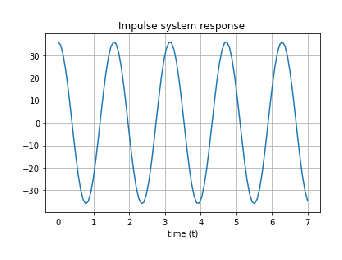
\includegraphics[width=\columnwidth]{./figs/es17btech11002/imp1.eps}
\caption{}
\label{fig:es17btech11002_imp1}
\end{figure}
\renewcommand{\thefigure}{\theenumi.\arabic{figure}}
%--------
The following python code plots the step response of the system. Fig.\ref{fig:es17btech11002_step1}.
\begin{lstlisting}
codes/es17btech11002/es17btech11002_step1.py
\end{lstlisting}
\begin{figure}[!ht]
\centering
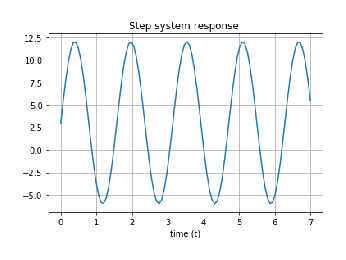
\includegraphics[width=\columnwidth]{./figs/es17btech11002/step1.eps}
\caption{}
\label{fig:es17btech11002_step1}
\end{figure}
\renewcommand{\thefigure}{\theenumi.\arabic{figure}}
%
\textbf{Amplitude:} From Fig. \ref{fig:es17btech11002_step1}  V \brak{peak-peak} is 
\begin{align}
V_{p-p} &= 11.929-(-5.957)= 17.886
\end{align}
\begin{align}
V_{max} &= \frac{V_{p-p}}{2} = 8.943
\end{align}
\textbf{Frequency:} From equation \eqref{eq:es17btech11002_freq}
\begin{align}
\omega = \frac{1}{RC} = 4 rad/sec
\end{align}
\begin{align}
f = \frac{\omega }{2\pi} = 0.636 Hz
\end{align}
\item Verify the frequency using spice simulation.\\
\solution The following readme file provides necessary instructions to simulate the circuit in spice.
\begin{lstlisting}
codes/es17btech11002/spice2/README
\end{lstlisting}
The following netlist simulates the given circuit.
\begin{lstlisting}
codes/es17btech11002/spice2/es17btech11002.net
\end{lstlisting}
The following code plots the output from the oscillator spice simulation which is shown in Fig. \ref{fig:es17btech11002_spice}.
\begin{lstlisting}
codes/es17btech11002/spice2/es17btech11002_2_spice.py
\end{lstlisting}
\renewcommand{\thefigure}{\theenumi.\arabic{figure}}
%
\begin{figure}[!ht]
\centering
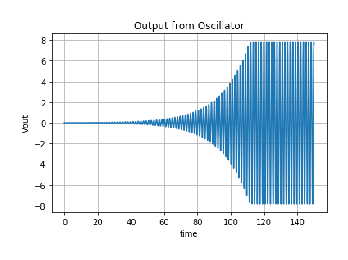
\includegraphics[width=\columnwidth]{./figs/es17btech11002/es17btech11002_2_spice.eps}
\caption{}
\label{fig:es17btech11002_spice}
\end{figure}
%
The following code plots a part of the spice output from which we can observe a clear sinusoidal output shown in Fig. \ref{fig:es17btech11002_spice2}.
\begin{lstlisting}
codes/es17btech11002/spice2/es17btech11002_spice2.py
\end{lstlisting}
\begin{figure}[!ht]
\centering
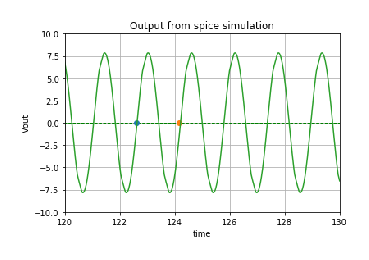
\includegraphics[width=\columnwidth]{./figs/es17btech11002/es17btech11002_2_spice2.eps}
\caption{}
\label{fig:es17btech11002_spice2}
\end{figure}
\renewcommand{\thefigure}{\theenumi}
%----------------------------------

\textbf{Amplitude:} From Fig. \ref{fig:es17btech11002_spice2} V(peak-peak) is 
\begin{align}
V_{p-p} &= 7.86-(-7.86) = 15.72
\end{align}
\begin{align}
V_{max} &= \frac{V_{p-p}}{2} = 7.86.
\end{align}
\textbf{Frequency:} time period is calculated by any two end points of one cycle,
\begin{align}
T&=124.150-(122.160) = 1.61 sec
\end{align}
\begin{align}
f = \frac{1}{T} = 0.64 Hz
\end{align}
Hence,the frequency is verified through the spice simulation.
%----------------------------------
\begin{table}[!ht]
\centering
%%%%%%%%%%%%%%%%%%%%%%%%%%%%%%%%%%%%%%%%%%%%%%%%%%%%%%%%%%%%%%%%%%%%%%
%%                                                                  %%
%%  This is the header of a LaTeX2e file exported from Gnumeric.    %%
%%                                                                  %%
%%  This file can be compiled as it stands or included in another   %%
%%  LaTeX document. The table is based on the longtable package so  %%
%%  the longtable options (headers, footers...) can be set in the   %%
%%  preamble section below (see PRAMBLE).                           %%
%%                                                                  %%
%%  To include the file in another, the following two lines must be %%
%%  in the including file:                                          %%
%%        \def\inputGnumericTable{}                                 %%
%%  at the beginning of the file and:                               %%
%%        \input{name-of-this-file.tex}                             %%
%%  where the table is to be placed. Note also that the including   %%
%%  file must use the following packages for the table to be        %%
%%  rendered correctly:                                             %%
%%    \usepackage[latin1]{inputenc}                                 %%
%%    \usepackage{color}                                            %%
%%    \usepackage{array}                                            %%
%%    \usepackage{longtable}                                        %%
%%    \usepackage{calc}                                             %%
%%    \usepackage{multirow}                                         %%
%%    \usepackage{hhline}                                           %%
%%    \usepackage{ifthen}                                           %%
%%  optionally (for landscape tables embedded in another document): %%
%%    \usepackage{lscape}                                           %%
%%                                                                  %%
%%%%%%%%%%%%%%%%%%%%%%%%%%%%%%%%%%%%%%%%%%%%%%%%%%%%%%%%%%%%%%%%%%%%%%



%%  This section checks if we are begin input into another file or  %%
%%  the file will be compiled alone. First use a macro taken from   %%
%%  the TeXbook ex 7.7 (suggestion of Han-Wen Nienhuys).            %%
\def\ifundefined#1{\expandafter\ifx\csname#1\endcsname\relax}


%%  Check for the \def token for inputed files. If it is not        %%
%%  defined, the file will be processed as a standalone and the     %%
%%  preamble will be used.                                          %%
\ifundefined{inputGnumericTable}

%%  We must be able to close or not the document at the end.        %%
	\def\gnumericTableEnd{\end{document}}


%%%%%%%%%%%%%%%%%%%%%%%%%%%%%%%%%%%%%%%%%%%%%%%%%%%%%%%%%%%%%%%%%%%%%%
%%                                                                  %%
%%  This is the PREAMBLE. Change these values to get the right      %%
%%  paper size and other niceties.                                  %%
%%                                                                  %%
%%%%%%%%%%%%%%%%%%%%%%%%%%%%%%%%%%%%%%%%%%%%%%%%%%%%%%%%%%%%%%%%%%%%%%

	\documentclass[12pt%
			  %,landscape%
                    ]{report}
       \usepackage[latin1]{inputenc}
       \usepackage{fullpage}
       \usepackage{color}
       \usepackage{array}
       \usepackage{longtable}
       \usepackage{calc}
       \usepackage{multirow}
       \usepackage{hhline}
       \usepackage{ifthen}

	\begin{document}


%%  End of the preamble for the standalone. The next section is for %%
%%  documents which are included into other LaTeX2e files.          %%
\else

%%  We are not a stand alone document. For a regular table, we will %%
%%  have no preamble and only define the closing to mean nothing.   %%
    \def\gnumericTableEnd{}

%%  If we want landscape mode in an embedded document, comment out  %%
%%  the line above and uncomment the two below. The table will      %%
%%  begin on a new page and run in landscape mode.                  %%
%       \def\gnumericTableEnd{\end{landscape}}
%       \begin{landscape}


%%  End of the else clause for this file being \input.              %%
\fi

%%%%%%%%%%%%%%%%%%%%%%%%%%%%%%%%%%%%%%%%%%%%%%%%%%%%%%%%%%%%%%%%%%%%%%
%%                                                                  %%
%%  The rest is the gnumeric table, except for the closing          %%
%%  statement. Changes below will alter the table's appearance.     %%
%%                                                                  %%
%%%%%%%%%%%%%%%%%%%%%%%%%%%%%%%%%%%%%%%%%%%%%%%%%%%%%%%%%%%%%%%%%%%%%%

\providecommand{\gnumericmathit}[1]{#1} 
%%  Uncomment the next line if you would like your numbers to be in %%
%%  italics if they are italizised in the gnumeric table.           %%
%\renewcommand{\gnumericmathit}[1]{\mathit{#1}}
\providecommand{\gnumericPB}[1]%
{\let\gnumericTemp=\\#1\let\\=\gnumericTemp\hspace{0pt}}
 \ifundefined{gnumericTableWidthDefined}
        \newlength{\gnumericTableWidth}
        \newlength{\gnumericTableWidthComplete}
        \newlength{\gnumericMultiRowLength}
        \global\def\gnumericTableWidthDefined{}
 \fi
%% The following setting protects this code from babel shorthands.  %%
 \ifthenelse{\isundefined{\languageshorthands}}{}{\languageshorthands{english}}
%%  The default table format retains the relative column widths of  %%
%%  gnumeric. They can easily be changed to c, r or l. In that case %%
%%  you may want to comment out the next line and uncomment the one %%
%%  thereafter                                                      %%
\providecommand\gnumbox{\makebox[0pt]}
%%\providecommand\gnumbox[1][]{\makebox}

%% to adjust positions in multirow situations                       %%
\setlength{\bigstrutjot}{\jot}
\setlength{\extrarowheight}{\doublerulesep}

%%  The \setlongtables command keeps column widths the same across  %%
%%  pages. Simply comment out next line for varying column widths.  %%
\setlongtables

\setlength\gnumericTableWidth{%
	53pt+%
	93pt+%
0pt}
\def\gumericNumCols{2}
\setlength\gnumericTableWidthComplete{\gnumericTableWidth+%
         \tabcolsep*\gumericNumCols*2+\arrayrulewidth*\gumericNumCols}
\ifthenelse{\lengthtest{\gnumericTableWidthComplete > \linewidth}}%
         {\def\gnumericScale{\ratio{\linewidth-%
                        \tabcolsep*\gumericNumCols*2-%
                        \arrayrulewidth*\gumericNumCols}%
{\gnumericTableWidth}}}%
{\def\gnumericScale{1}}

%%%%%%%%%%%%%%%%%%%%%%%%%%%%%%%%%%%%%%%%%%%%%%%%%%%%%%%%%%%%%%%%%%%%%%
%%                                                                  %%
%% The following are the widths of the various columns. We are      %%
%% defining them here because then they are easier to change.       %%
%% Depending on the cell formats we may use them more than once.    %%
%%                                                                  %%
%%%%%%%%%%%%%%%%%%%%%%%%%%%%%%%%%%%%%%%%%%%%%%%%%%%%%%%%%%%%%%%%%%%%%%

\ifthenelse{\isundefined{\gnumericColA}}{\newlength{\gnumericColA}}{}\settowidth{\gnumericColA}{\begin{tabular}{@{}p{53pt*\gnumericScale}@{}}x\end{tabular}}
\ifthenelse{\isundefined{\gnumericColB}}{\newlength{\gnumericColB}}{}\settowidth{\gnumericColB}{\begin{tabular}{@{}p{93pt*\gnumericScale}@{}}x\end{tabular}}

\begin{tabular}[c]{%
	b{\gnumericColA}%
	b{\gnumericColB}%
	}

%%%%%%%%%%%%%%%%%%%%%%%%%%%%%%%%%%%%%%%%%%%%%%%%%%%%%%%%%%%%%%%%%%%%%%
%%  The longtable options. (Caption, headers... see Goosens, p.124) %%
%	\caption{The Table Caption.}             \\	%
% \hline	% Across the top of the table.
%%  The rest of these options are table rows which are placed on    %%
%%  the first, last or every page. Use \multicolumn if you want.    %%

%%  Header for the first page.                                      %%
%	\multicolumn{2}{c}{The First Header} \\ \hline 
%	\multicolumn{1}{c}{colTag}	%Column 1
%	&\multicolumn{1}{c}{colTag}	\\ \hline %Last column
%	\endfirsthead

%%  The running header definition.                                  %%
%	\hline
%	\multicolumn{2}{l}{\ldots\small\slshape continued} \\ \hline
%	\multicolumn{1}{c}{colTag}	%Column 1
%	&\multicolumn{1}{c}{colTag}	\\ \hline %Last column
%	\endhead

%%  The running footer definition.                                  %%
%	\hline
%	\multicolumn{2}{r}{\small\slshape continued\ldots} \\
%	\endfoot

%%  The ending footer definition.                                   %%
%	\multicolumn{2}{c}{That's all folks} \\ \hline 
%	\endlastfoot
%%%%%%%%%%%%%%%%%%%%%%%%%%%%%%%%%%%%%%%%%%%%%%%%%%%%%%%%%%%%%%%%%%%%%%

\hhline{|-|-}
	 \multicolumn{1}{|p{\gnumericColA}|}%
	{\gnumericPB{\centering}\gnumbox{\textbf{Parameter}}}
	&\multicolumn{1}{p{\gnumericColB}|}%
	{\gnumericPB{\centering}\gnumbox{\textbf{Value}}}
\\
\hhline{|--|}
	 \multicolumn{1}{|p{\gnumericColA}|}%
	{\gnumericPB{\centering}\gnumbox{$R$}}
	&\multicolumn{1}{p{\gnumericColB}|}%
	{$10 \Omega$}
\\
\hhline{|--|}
	 \multicolumn{1}{|p{\gnumericColA}|}%
	{\gnumericPB{\centering}\gnumbox{$C$}}
	&\multicolumn{1}{p{\gnumericColB}|}%
	{$0.01mF$}
\\
\hhline{|-|-|}
	 \multicolumn{1}{|p{\gnumericColA}|}%
	{\gnumericPB{\centering}\gnumbox{$R_{1}$}}
	&\multicolumn{1}{p{\gnumericColB}|}%
	{$1000\Omega $}
\\
\hhline{|--|}
	 \multicolumn{1}{|p{\gnumericColA}|}%
	{\gnumericPB{\centering}\gnumbox{$R_{2}$}}
	&\multicolumn{1}{p{\gnumericColB}|}%
	{$2030\Omega $}	
\\
\hhline{|-|-|}
\end{tabular}

\ifthenelse{\isundefined{\languageshorthands}}{}{\languageshorthands{\languagename}}
\gnumericTableEnd
\caption{}
\label{table:es17btech11002_Input_Table2}
\end{table}
\renewcommand{\thefigure}{\theenumi.\arabic{figure}}


\item Now find the Amplitude and frequency for some arbitrary R, C values given in Table \ref{table:es17btech11002_Input_Table2}.\\

\solution The following python code plots the step response of the system. Fig. \ref{fig:es17btech11002_step2}.
\begin{figure}[!ht]
\centering
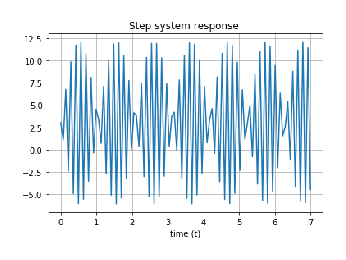
\includegraphics[width=\columnwidth]{./figs/es17btech11002/step2.eps}
\caption{}
\label{fig:es17btech11002_step2}
\end{figure}
\begin{lstlisting}
codes/es17btech11002/es17btech11002_step2.py
\end{lstlisting}
The following python code plots the impulse response of the system Fig. \ref{fig:es17btech11002_imp2}.
\begin{lstlisting}
codes/es17btech11002/es17btech11002_imp2.py
\end{lstlisting}
\begin{figure}[!ht]
\centering
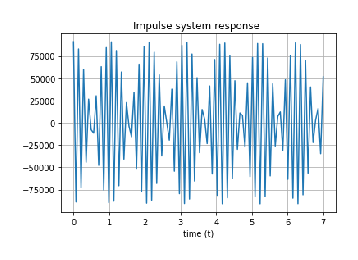
\includegraphics[width=\columnwidth]{./figs/es17btech11002/imp2.eps}
\caption{}
\label{fig:es17btech11002_imp2}
\end{figure}

\textbf{Frequency:} From equation \eqref{eq:es17btech11002_freq}
\begin{align}
\omega = \frac{1}{RC} = 10000 rad/sec
\end{align}
\begin{align}
f = \frac{\omega }{2\pi} = 1.57 kHz
\end{align}
\item Now again verify the frequency using spice simulation.\\
\solution The following readme file provides necessary instructions to simulate the circuit in spice.
\begin{lstlisting}
codes/es17btech11002/spice/README
\end{lstlisting}
The following netlist simulates the given circuit.
\begin{lstlisting}
codes/es17btech11002/spice/es17btech11002.net
\end{lstlisting}
The following code plots the output from the oscillator spice simulation which is shown in Fig. \ref{fig:es17btech11002_2_spice}.
\begin{lstlisting}
codes/es17btech11002/spice/es17btech11002_spice.py
\end{lstlisting}
\renewcommand{\thefigure}{\theenumi.\arabic{figure}}
%
\begin{figure}[!ht]
\centering
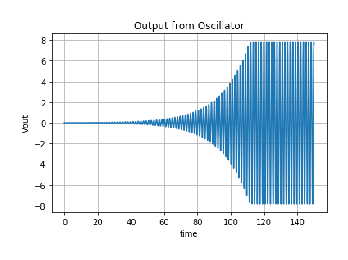
\includegraphics[width=\columnwidth]{./figs/es17btech11002/es17btech11002_spice.eps}
\caption{}
\label{fig:es17btech11002_2_spice}
\end{figure}
%
The following code plots a part of the spice output from Fig \ref{fig:es17btech11002_2_spice}. which we can observe a clear sinusoidal output shown in Fig. \ref{fig:es17btech11002_spice4}.
\begin{lstlisting}
codes/es17btech11002/spice/es17btech11002_spice2.py
\end{lstlisting}
\begin{figure}[!ht]
\centering
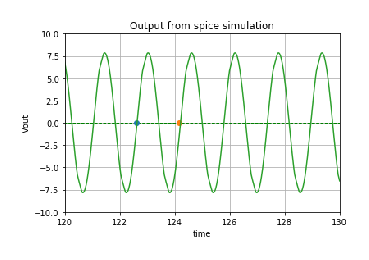
\includegraphics[width=\columnwidth]{./figs/es17btech11002/es17btech11002_spice2.eps}
\caption{}
\label{fig:es17btech11002_spice4}
\end{figure}
\renewcommand{\thefigure}{\theenumi}
\textbf{Amplitude:}From Fig. \ref{fig:es17btech11002_spice4} V(peak-peak) is 
\begin{align}
V_{p-p} &= 0.47-(-0.47) = 0.94V
\end{align}
\begin{align}
V_{max} &= \frac{V_{p-p}}{2} = 0.47.
\end{align}
\textbf{Frequency:} time period is calculated by any two end points of one cycle,
\begin{align}
T&=0.0313164 - \brak{0.03060} = 0.7164 ms
\end{align}
\begin{align}
f = \frac{1}{T} = 1.39 kHz
\end{align}
Hence,the frequency is verified through the spice simulation.
\\
\textbf{NOTE :} Generally in real life scenario oscillator generate a sinusoidal signal by consuming the thermal noise in the circuit. So in the above two experiment it can be observed that in python simulation requires an input to generates the output as there is no thermal noise, it should also be noticed that beside amplitude the frequency in the python and spice simulation are almost same.  
\end{enumerate}
